\documentclass{article}
\usepackage[T1]{fontenc}
\usepackage{helvet}
\renewcommand{\familydefault}{\sfdefault}
\usepackage{amsmath,amssymb}
\usepackage{sansmath}
\usepackage{tikz}
\usetikzlibrary{arrows.meta,positioning}
\pagestyle{empty}
\definecolor{acc}{HTML}{1F4E79}
\newsavebox{\figbox}
\newcommand{\DD}{\mathord{\text{\fontencoding{OT1}\fontfamily{cmss}\selectfont\char1}}}
\begin{document}
\sansmath\fontsize{7}{8.4}\selectfont
\sbox{\figbox}{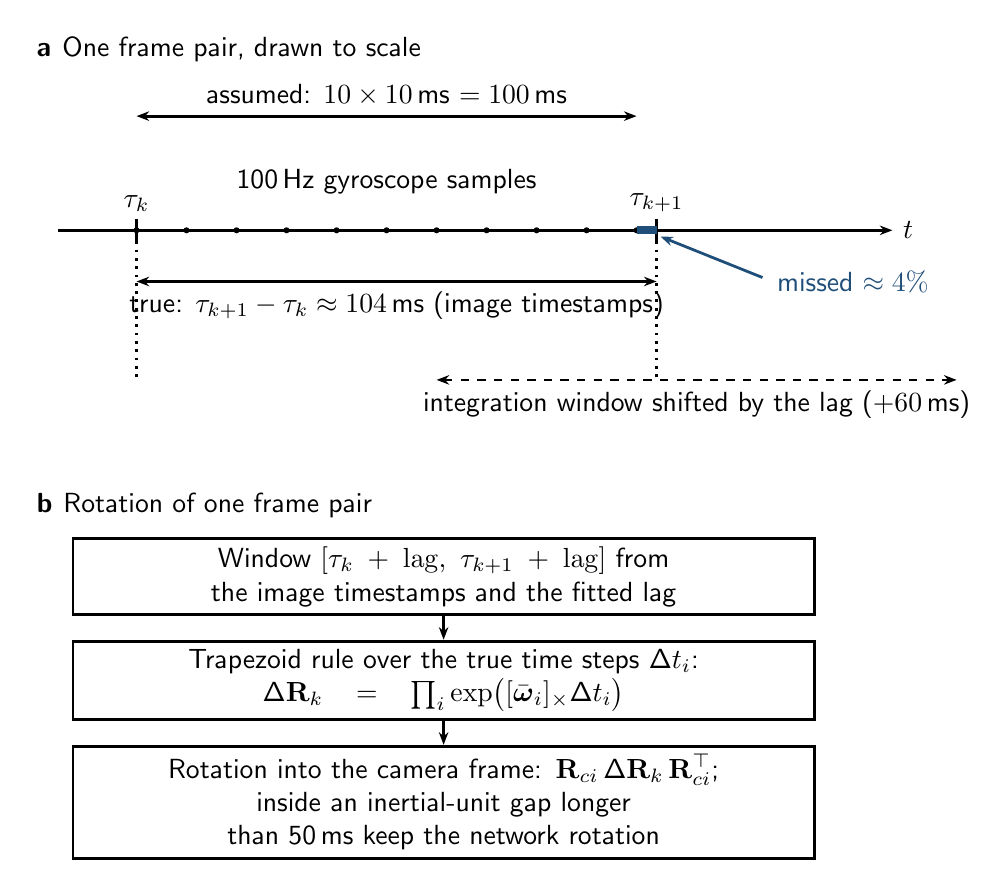
\begin{tikzpicture}[>={Stealth[length=1.6mm]}, every path/.style={line width=1pt},
  st/.style={draw, align=center, inner sep=3pt, text width=9.2cm}]
% scale: 1 ms = 0.0635 cm
\def\s{0.0635}
\node[anchor=west] at (-0.4,2.3) {\textbf{a}\hspace{4pt}One frame pair, drawn to scale};
\draw[->] (0,0) -- (10.6,0) node[right] {$t$};
\foreach \j in {0,...,10} {\fill ({1.0+10*\s*\j},0) circle (1.1pt);}
\node at ({1.0+50*\s},0.62) {100\,Hz gyroscope samples};
\draw (1.0,-0.14) -- (1.0,0.14); \node[above] at (1.0,0.1) {$\tau_k$};
\draw ({1.0+104*\s},-0.14) -- ({1.0+104*\s},0.14); \node[above] at ({1.0+104*\s},0.1) {$\tau_{k+1}$};
\draw[acc, line width=3pt] ({1.0+100*\s},0) -- ({1.0+104*\s},0);
\draw[<->] (1.0,1.45) -- ({1.0+100*\s},1.45) node[midway, above] {assumed: $10\times10$\,ms $=100$\,ms};
\node[acc, anchor=west] at (9.0,-0.65) {missed $\approx4\%$};
\draw[acc, ->] (8.95,-0.6) -- ({1.0+104*\s+0.05},-0.08);
\draw[<->] (1.0,-0.65) -- ({1.0+104*\s},-0.65) node[midway, below] {true: $\tau_{k+1}-\tau_k\approx104$\,ms (image timestamps)};
\draw[dotted] (1.0,-0.14) -- (1.0,-1.9); \draw[dotted] ({1.0+104*\s},-0.14) -- ({1.0+104*\s},-1.9);
\draw[<->, dashed] ({1.0+60*\s},-1.9) -- ({1.0+164*\s},-1.9) node[midway, below] {integration window shifted by the lag ($+60$\,ms)};
\node[anchor=west] at (-0.4,-3.5) {\textbf{b}\hspace{4pt}Rotation of one frame pair};
\node[st] (s1) at (4.9,-4.4) {Window $[\tau_k+\mathrm{lag},\ \tau_{k+1}+\mathrm{lag}]$ from the image timestamps and the fitted lag};
\node[st, below=3mm of s1] (s2) {Trapezoid rule over the true time steps $\DD t_i$:\\ $\DD\mathbf{R}_k=\prod_i \exp\!\big([\bar{\boldsymbol\omega}_i]_\times \DD t_i\big)$};
\node[st, below=3mm of s2] (s3) {Rotation into the camera frame: $\mathbf{R}_{ci}\,\DD\mathbf{R}_k\,\mathbf{R}_{ci}^{\top}$;\\ inside an inertial-unit gap longer than 50\,ms keep the network rotation};
\draw[->] (s1) -- (s2); \draw[->] (s2) -- (s3);
\end{tikzpicture}}
\hoffset=-1in \voffset=-1in
\pdfpagewidth=\wd\figbox
\pdfpageheight=\ht\figbox \advance\pdfpageheight by \dp\figbox
\shipout\copy\figbox
\end{document}
